%Autor: Simon Walker
%Version: 1.0
%Datum: 18.04.2020
%Lizenz: CC BY-NC-SA

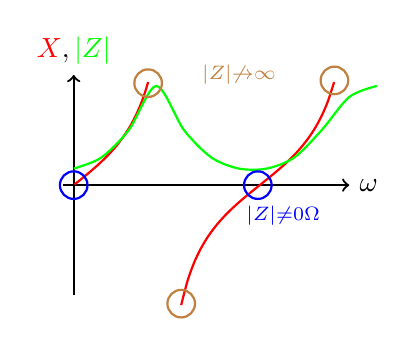
\begin{tikzpicture}[smooth, xscale=0.7, yscale=0.7]
% Achsen
\draw[->, thick] (-0.2,0) -- +(5.2,0) node[right] {$\omega$}; % Horizontal
\draw[->, thick] (0,-2) -- +(0,4) node[above] {$\color{red}X \color{black}, \color{green} \left|Z\right|$}; % Vertikal

% Plots
\draw[color=red, thick] plot[domain=0.01:0.9] (\x*1.5,{tan((\x *1.2) r )}); % Erster Tan
\draw[color=red, thick] plot[domain=1.3:3.15] (\x*1.5,{tan((\x*1.2 -2.7) r)}); % Zweiter Tan
%Impedanz
%\draw[color=green, thick] plot[domain=0.01:0.9] (\x*1.5,{0.3+0.6*tan((\x *1.2) r )}); % Erster Tan

\draw [green, thick] plot [smooth] coordinates{
(0, 0.3) (0.5, 0.5) (1, 1) 
(1.5, 1.8)  (2, 1) (2.5, 0.5)
(3, 0.3) (3.5, 0.3) (4, 0.5) 
(4.5, 1) (5, 1.6) (5.5, 1.8)};


\draw [blue, thick] (3.34, 0) circle[radius=0.25];
\draw [blue, thick] (0, 0) circle[radius=0.25];
\draw [brown, thick] (1.35, 1.85) circle[radius=0.25];
\draw [brown, thick] (1.95, -2.15) circle[radius=0.25];
\draw [brown, thick] (4.73, 1.9) circle[radius=0.25];

\node [below] at (3.8, -0.2) {$\scriptstyle \color{blue} \left|Z\right| \ne 0 \Omega$};
\node at (3, 2) {$\scriptstyle \color{brown} \left|Z\right| \not\rightarrow \infty$};

\end{tikzpicture}